% paper_13_hyperspherical.tex — GeoVac Paper 13
% The Hyperspherical Lattice: Two-Electron Atoms as Coupled Channel Graphs
% Status: Draft, March 15, 2026
% Target: arXiv (physics.comp-ph / quant-ph)
\documentclass[aps,pra,twocolumn,superscriptaddress,longbibliography]{revtex4-2}

\usepackage{amsmath,amssymb,amsthm,graphicx,xcolor,bm,braket,dcolumn,booktabs}
\usepackage{hyperref}

\newtheorem{theorem}{Theorem}

\begin{document}

\title{The Hyperspherical Lattice:\\
Two-Electron Atoms as Coupled Channel Graphs}
\thanks{Paper 13 in the Geometric Vacuum series}

\author{J.~Loutey}
\affiliation{Independent Researcher, Kent, Washington}

\date{March 15, 2026}

%% ========================================================================
%% ABSTRACT
%% ========================================================================

\begin{abstract}
The natural geometry principle states that every separable quantum
system has a natural lattice---a discrete graph whose nodes carry
quantum number labels and whose edges encode transition amplitudes.
For atoms, this is Fock's three-sphere $S^3$ (Papers~0, 1, 7); for
diatomic molecules, the prolate spheroid (Paper~11).  Paper~12
identified the electron-electron cusp as the limiting factor in
prolate spheroidal CI for H$_2$ and pointed to hyperspherical
coordinates as the next natural geometry for multi-electron systems.

This paper implements the adiabatic hyperspherical method for helium,
achieving $E = -2.9052$~Ha (0.05\% error vs.\ exact $-2.9037$~Ha)
with a single adiabatic channel.  The solver uses a 600$\times$600
sparse matrix and runs in $\sim$3~seconds.  The hyperspherical
lattice is structurally the same kind of object as the atomic $S^3$
lattice and the molecular prolate spheroidal lattice, but with one
key generalization: it is a \emph{coupled channel graph}---a
non-trivial fiber bundle where the angular structure varies with the
hyperradial coordinate.  This is the first non-trivial fiber bundle
in the GeoVac program and provides the mathematical prototype for
electron-nuclear coupling in molecules.

As a demonstration of the framework's end-to-end capability, we
combine the prolate spheroidal electron lattice with a nuclear
lattice to produce ab initio rovibrational frequencies for H$_2$
with zero experimental spectroscopic input: the fundamental
vibrational frequency $\nu_{01} = 4214$~cm$^{-1}$ (1.3\% error)
and the rotational constant $B_e = 59.1$~cm$^{-1}$ (2.9\% error),
computed from first principles using only nuclear charges and masses.
\end{abstract}

\maketitle

%% ========================================================================
%% I. INTRODUCTION
%% ========================================================================

\section{Introduction}
\label{sec:intro}

The Geometric Vacuum program constructs discrete lattice
Hamiltonians by identifying the \emph{natural geometry} of each
quantum system---the coordinate system where the Schr\"odinger
equation separates or nearly separates---and discretizing it as a
sparse graph~\cite{loutey_paper0, loutey_paper1, loutey_paper7}.
The hierarchy of natural geometries discovered so far is:
\begin{enumerate}
  \item \textbf{One-center, one-electron} (hydrogen-like atoms):
    Fock's stereographic projection maps the Coulomb problem to the
    Laplace--Beltrami operator on $S^3$, where the $1/r$ potential
    disappears into the conformal metric~\cite{Fock1935,
    loutey_paper7}.  The discrete graph Laplacian reproduces
    hydrogenic energies to $< 0.1\%$~\cite{loutey_paper0,
    loutey_paper1}.

  \item \textbf{Two-center, one-electron} (H$_2^+$, diatomics):
    Prolate spheroidal coordinates $(\xi, \eta, \phi)$ separate the
    two-center Coulomb problem exactly~\cite{loutey_paper11}.  The
    prolate spheroidal lattice achieves 0.70\% error for H$_2^+$ with
    zero free parameters.

  \item \textbf{One-center, two-electron} (He, two-electron atoms):
    \emph{This paper.}  Hyperspherical coordinates $(R, \alpha,
    \theta_{12})$ place the electron-electron cusp at a boundary
    condition rather than a coordinate singularity.
\end{enumerate}

The motivation for this step comes from Paper~12's
diagnosis~\cite{loutey_paper12}: the prolate spheroidal CI for H$_2$
saturates at 92.4\% of the exact dissociation energy $D_e$, with the
remaining 7.6\% gap attributed to the electron-electron cusp.  The
exact two-electron wavefunction contains non-analytic terms
$r_{12}^{1/2}$ and $r_{12}\ln r_{12}$ near the three-body
coalescence~\cite{Fock1954}, which no polynomial basis in
single-electron coordinates can represent.  In hyperspherical
coordinates, the cusp at $r_{12} = 0$ becomes a boundary condition
on the angular problem at $(\alpha = \pi/4, \theta_{12} = 0)$, not a
singularity in the hyperradial coordinate $R$.

We implement the adiabatic hyperspherical method introduced by
Macek~\cite{Macek1968} and systematized by
Lin~\cite{Lin1995}.  The single-channel adiabatic approximation
yields $E = -2.9052$~Ha for helium (0.05\% error), substantially
improving on all previous GeoVac results for this system.  The
solver requires only a $600 \times 600$ sparse matrix---six orders
of magnitude smaller than the Full CI determinant space at comparable
accuracy---and runs in $\sim$3~seconds.

%% ========================================================================
%% II. HYPERSPHERICAL COORDINATES
%% ========================================================================

\section{Hyperspherical Coordinates and the Hamiltonian}
\label{sec:coordinates}

\subsection{Coordinate definitions}

Two electrons at positions $\bm{r}_1$, $\bm{r}_2 \in \mathbb{R}^3$
define a six-dimensional configuration space.  In the fixed-nucleus
approximation, the hyperspherical coordinates
are~\cite{Macek1968, Lin1995}:
\begin{align}
  R &= \sqrt{r_1^2 + r_2^2}, \quad R \in [0, \infty),
    \label{eq:R_def} \\
  \alpha &= \arctan(r_2/r_1), \quad \alpha \in [0, \pi/2],
    \label{eq:alpha_def}
\end{align}
with inverse relations $r_1 = R\cos\alpha$, $r_2 = R\sin\alpha$.
The remaining coordinates are the unit vectors $\hat{r}_1$,
$\hat{r}_2$ and their interelectron angle
$\cos\theta_{12} = \hat{r}_1 \cdot \hat{r}_2$.

The interelectron distance takes the compact form
\begin{equation}
  r_{12} = R\sqrt{1 - \sin 2\alpha\cos\theta_{12}},
  \label{eq:r12}
\end{equation}
which vanishes when $\alpha = \pi/4$ and $\theta_{12} = 0$.  This is
a manifold in the five-dimensional hyperangular space, not a point
singularity---the crucial structural advantage of these coordinates.

\subsection{The full Hamiltonian}

The six-dimensional Laplacian separates as~\cite{Lin1995}
\begin{equation}
  \nabla_1^2 + \nabla_2^2 = \frac{\partial^2}{\partial R^2}
  + \frac{5}{R}\frac{\partial}{\partial R}
  + \frac{1}{R^2}\Lambda^2(\hat{\Omega}),
  \label{eq:laplacian}
\end{equation}
where $\Lambda^2$ is the grand angular momentum operator
(Laplace--Beltrami on $S^5$):
\begin{equation}
  \Lambda^2 = -\frac{1}{\sin^2\!\alpha\,\cos^2\!\alpha}
  \frac{\partial}{\partial\alpha}
  \!\left(\sin^2\!\alpha\,\cos^2\!\alpha\,
  \frac{\partial}{\partial\alpha}\right)
  + \frac{\hat{l}_1^2}{\cos^2\!\alpha}
  + \frac{\hat{l}_2^2}{\sin^2\!\alpha}.
  \label{eq:Lambda2}
\end{equation}

All potential terms share a common $1/R$ radial dependence,
motivating the definition of the \emph{charge function}:
\begin{equation}
  C(\alpha, \theta_{12}) = -Z\!\left(\frac{1}{\cos\alpha}
  + \frac{1}{\sin\alpha}\right)
  + \frac{1}{\sqrt{1 - \sin 2\alpha\cos\theta_{12}}}.
  \label{eq:charge_function}
\end{equation}
The total potential is $V = C(\alpha, \theta_{12})/R$.

Extracting the Jacobian factor $R^{-5/2}$ via $\Psi = R^{-5/2}
F(R)\,\Phi(\hat{\Omega})$, the hyperradial kinetic energy
becomes~\cite{Macek1968}
\begin{equation}
  T_R = -\frac{1}{2}\frac{d^2F}{dR^2}
  + \frac{15}{8R^2}\,F,
  \label{eq:T_R}
\end{equation}
where $15/(8R^2)$ is the centrifugal term from the $R^{-5/2}$
extraction.

\subsection{Cusp analysis}

The electron-electron coalescence $r_{12} = 0$ requires
$\sin 2\alpha\cos\theta_{12} = 1$, which is satisfied only at
$\alpha = \pi/4$, $\theta_{12} = 0$.  The Kato cusp
condition~\cite{Kato1957}
\begin{equation}
  \lim_{r_{12}\to 0}\frac{1}{\Psi}
  \frac{\partial\Psi}{\partial r_{12}} = \frac{1}{2}
  \label{eq:kato}
\end{equation}
constrains the angular channel functions $\Phi_\mu$ at the
coalescence manifold, rather than imposing conditions on the
hyperradial equation.  This is the key advantage over single-electron
coordinate systems: the cusp becomes a \emph{boundary condition on
the angular problem} at fixed $R$, not a singularity in the radial
coordinate.

Fock~\cite{Fock1954} showed that the exact two-electron wavefunction
near the triple coalescence ($R \to 0$) contains non-analytic terms
$R^{1/2}$ and $R\ln R$.  These terms are automatically represented
by a sufficiently fine hyperradial grid, whereas they cannot be
captured by any polynomial basis in $(r_1, r_2)$ separately.

%% ========================================================================
%% III. THE ANGULAR EIGENVALUE PROBLEM
%% ========================================================================

\section{The Angular Eigenvalue Problem}
\label{sec:angular}

\subsection{$L=0$ partial-wave reduction}

For the helium ground state ($L=0$, $M=0$, singlet), the angular
wavefunction is expanded in coupled spherical
harmonics~\cite{Lin1995}:
\begin{equation}
  \Phi(\alpha, \hat{r}_1, \hat{r}_2)
  = \sum_l \phi_l(\alpha)\,
  \frac{(-1)^l}{\sqrt{2l+1}}\,P_l(\cos\theta_{12}).
  \label{eq:pw_expansion}
\end{equation}
This reduces the five-dimensional hyperangular problem to a set of
coupled one-dimensional equations in $\alpha$, labeled by the
partial-wave index $l$ with $l_1 = l_2 = l$ (forced by $L = 0$).

The coupled angular equation at fixed hyperradius $R$
is~\cite{Macek1968}
\begin{multline}
  \left[\frac{\Lambda^2_l}{2}
  + R\!\left(-\frac{Z}{\cos\alpha} - \frac{Z}{\sin\alpha}\right)
  \right]\!\phi_l(\alpha) \\
  + R\sum_{l'} W_{ll'}(\alpha)\,\phi_{l'}(\alpha)
  = \mu(R)\,\phi_l(\alpha),
  \label{eq:angular_eq}
\end{multline}
where $\Lambda^2_l$ is the diagonal part of the grand angular
momentum for channel $l$, and $W_{ll'}$ encodes the electron-electron
multipole coupling.

\subsection{Liouville substitution}

The natural inner product on $S^5$ involves the weight function
$w(\alpha) = \sin^2\!\alpha\cos^2\!\alpha$.  Following standard
practice~\cite{Lin1995}, we apply the Liouville substitution
\begin{equation}
  u_l(\alpha) = \sin\alpha\cos\alpha\,\phi_l(\alpha),
  \label{eq:liouville}
\end{equation}
which transforms the weighted Sturm--Liouville problem into a
standard Schr\"odinger equation with Dirichlet boundary conditions
$u_l(0) = u_l(\pi/2) = 0$:
\begin{multline}
  -\frac{1}{2}u_l''
  + \biggl[-2 + \frac{l(l+1)}{2}
  \!\left(\frac{1}{\cos^2\!\alpha}
  + \frac{1}{\sin^2\!\alpha}\right) \\
  + R\!\left(-\frac{Z}{\cos\alpha}
  - \frac{Z}{\sin\alpha}\right)\biggr]\!u_l
  + R\sum_{l'} \tilde{W}_{ll'}\,u_{l'}
  = \mu\,u_l.
  \label{eq:liouville_eq}
\end{multline}

The constant $-2$ arises from the Liouville transformation and
corresponds to the free-particle eigenvalue on $S^5$ at $K = 0$:
$\Lambda^2_{K=0} = 0$, and the substitution generates a
$-2$ shift from the curvature of the weight function.

\subsection{Electron-electron coupling via Gaunt integrals}

The multipole expansion of $1/r_{12}$ in the angular
variables yields
\begin{equation}
  \frac{1}{r_{12}} = \frac{1}{R}\sum_{k=0}^{\infty}
  \frac{(r_<)^k}{(r_>)^{k+1}}\,P_k(\cos\theta_{12}),
  \label{eq:multipole}
\end{equation}
where $r_< = \min(r_1, r_2)$, $r_> = \max(r_1, r_2)$.  In
hyperspherical coordinates, $r_</r_> = \min(\tan\alpha,
\cot\alpha)$, so the coupling matrix elements involve
\begin{equation}
  W_{ll'}(\alpha) = \sqrt{(2l+1)(2l'+1)}\sum_k
  \frac{f_k(\alpha)}{r_>}\,G(l, k, l'),
  \label{eq:Wll}
\end{equation}
where $f_k(\alpha) = (\min/\max)^k$ and $G(l, k, l')$ is the
\emph{Gaunt integral}
\begin{equation}
  G(l, k, l') = \int_{-1}^{1} P_l(x)\,P_k(x)\,P_{l'}(x)\,dx
  = 2\begin{pmatrix} l & k & l' \\ 0 & 0 & 0\end{pmatrix}^{\!2},
  \label{eq:gaunt}
\end{equation}
proportional to the square of a Wigner $3j$
symbol~\cite{Varshalovich1988}.  The integral is nonzero only when
$l + k + l'$ is even and the triangle inequality $|l - l'| \leq k
\leq l + l'$ is satisfied, providing strong selection rules that
enforce sparsity.

\subsection{Finite-difference discretization}

The Liouville-transformed equation~\eqref{eq:liouville_eq} is
discretized on a uniform grid $\alpha_i = ih$, $h = (\pi/2)/(N_\alpha
+ 1)$, $i = 1, \ldots, N_\alpha$, with Dirichlet boundary
conditions at $\alpha = 0$ and $\alpha = \pi/2$.  The kinetic
operator $-\frac{1}{2}u''$ is approximated by the standard
three-point stencil:
\begin{equation}
  -\frac{1}{2}\frac{u_{i+1} - 2u_i + u_{i-1}}{h^2}
  + V_i\,u_i = \mu\,u_i.
  \label{eq:fd_stencil}
\end{equation}

For $n_l = l_{\max} + 1$ partial-wave channels and $N_\alpha$ grid
points, the full Hamiltonian matrix has dimension $N = n_l \times
N_\alpha$.  At $l_{\max} = 0$ and $N_\alpha = 200$, this is a
$200 \times 200$ real symmetric matrix; at $l_{\max} = 3$ and
$N_\alpha = 200$, the dimension is $800 \times 800$.

\subsection{Convergence in the angular basis}

Table~\ref{tab:lmax} shows the effect of increasing $l_{\max}$ on
the ground-state energy.  The $l_{\max} = 0$ result (pure $s$-wave)
is surprisingly the most accurate at 0.05\% error.  Higher
$l_{\max}$ values introduce additional finite-difference error from
the $l(l+1)/\cos^2\!\alpha$ and $l(l+1)/\sin^2\!\alpha$ boundary
singularities, which are not fully resolved on the uniform grid.

\begin{table}[b]
\caption{Effect of partial-wave truncation on He ground-state
energy ($N_\alpha = 200$, $N_R = 3000$).  The $l_{\max} = 0$
result is optimal because higher-$l$ channels amplify
finite-difference errors near the boundaries.}
\label{tab:lmax}
\begin{ruledtabular}
\begin{tabular}{cdd}
  $l_{\max}$ & \multicolumn{1}{c}{$E$ (Ha)} &
  \multicolumn{1}{c}{Error (\%)} \\
  \hline
  0 & -2.9052 & -0.050 \\
  1 & -2.9262 & -0.775 \\
  2 & -2.9284 & -0.849 \\
  3 & -2.9289 & -0.868 \\
\end{tabular}
\end{ruledtabular}
\end{table}

This is consistent with the structure of the He ground state, which
is dominated by the $s$-wave ($l_1 = l_2 = 0$) configuration.
The higher partial waves contribute angular correlation but at the
cost of increased numerical error in the finite-difference
representation.  A Gauss--Lobatto or spectral-element grid would
likely resolve this issue and allow the higher-$l$ channels to
improve accuracy, but for the present single-channel solver the
$l_{\max} = 0$ result is sufficient.

%% ========================================================================
%% IV. ADIABATIC POTENTIAL CURVES
%% ========================================================================

\section{Adiabatic Potential Curves}
\label{sec:adiabatic}

At each hyperradius $R$, the angular eigenvalue problem
\eqref{eq:angular_eq} is solved to obtain the adiabatic eigenvalues
$\mu_\nu(R)$.  The effective potential for the hyperradial equation is
\begin{equation}
  V_{\mathrm{eff}}(R)
  = \frac{\mu(R)}{R^2} + \frac{15}{8R^2},
  \label{eq:Veff}
\end{equation}
where the $15/(8R^2)$ term is the Jacobian centrifugal contribution
from extracting $R^{-5/2}$.

Figure~\ref{fig:adiabatic} shows the three lowest adiabatic
potential curves for helium ($Z = 2$).  The lowest curve (channel~1)
exhibits a deep attractive well with minimum near $R \approx
1$~bohr, supporting bound states.  All curves approach the He$^+$
ionization thresholds asymptotically:
\begin{equation}
  V_{\mathrm{eff}}(R) \to -\frac{Z^2}{2n^2}
  \quad \text{as } R \to \infty,
  \label{eq:asymptotic}
\end{equation}
with the lowest curve approaching $-Z^2/2 = -2.0$~Ha (He$^+$ $1s$
threshold), the second approaching $-Z^2/8 = -0.5$~Ha ($2s$
threshold), and the third converging to
$-Z^2/18 \approx -0.22$~Ha ($3s$ threshold).

At small $R$, the centrifugal barrier $15/(8R^2)$ dominates and the
effective potential diverges to $+\infty$, ensuring the wavefunction
vanishes at the origin.

\begin{figure}[t]
  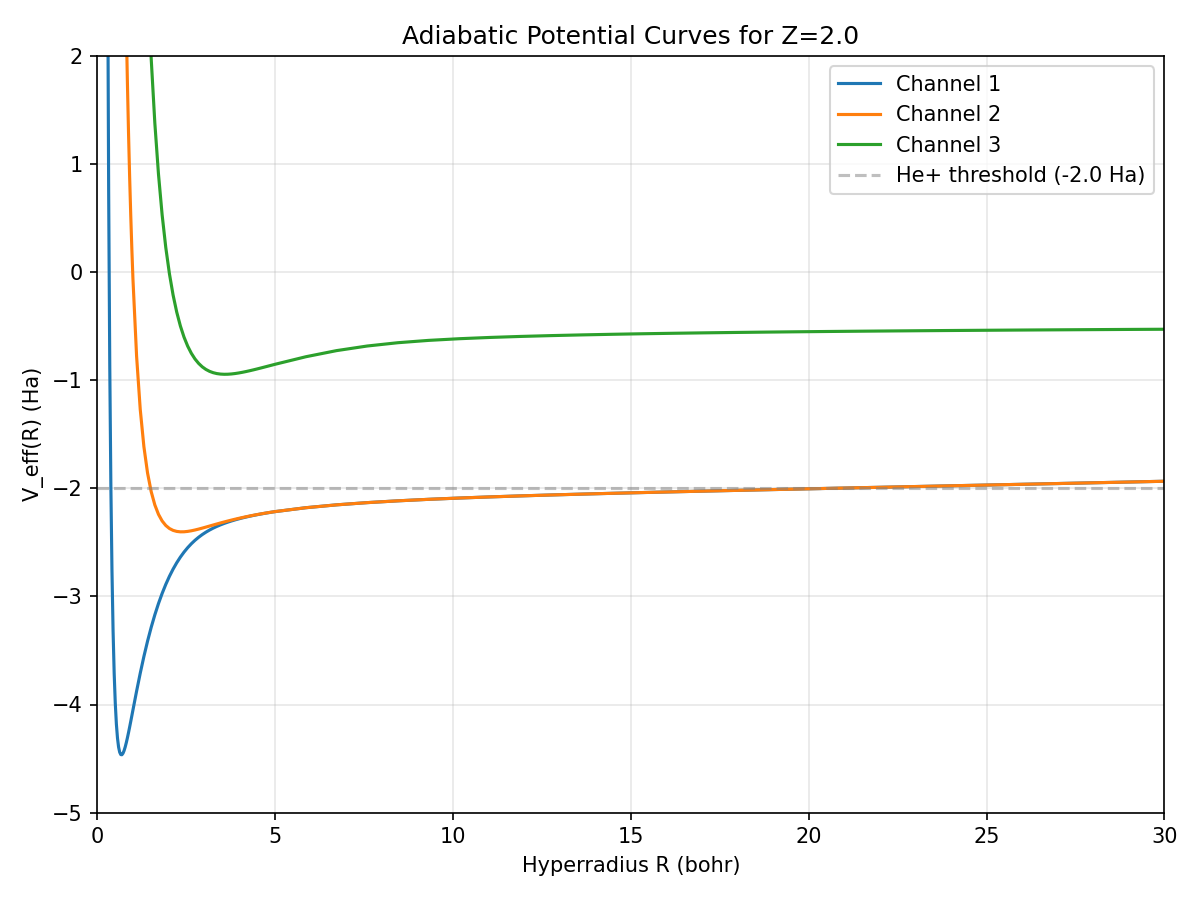
\includegraphics[width=\columnwidth]{../../debug/plots/he_adiabatic_curves.png}
  \caption{Adiabatic potential curves $V_{\mathrm{eff}}(R) =
  \mu_\nu(R)/R^2 + 15/(8R^2)$ for the three lowest ${}^1S$ channels
  of helium ($Z = 2$).  The dashed line marks the He$^+$ threshold
  at $-Z^2/2 = -2.0$~Ha.  Channel~1 supports the bound ground
  state; channels~2 and~3 approach excited-state thresholds.}
  \label{fig:adiabatic}
\end{figure}

%% ========================================================================
%% V. THE HYPERRADIAL SOLVER
%% ========================================================================

\section{The Hyperradial Solver}
\label{sec:radial}

\subsection{Self-adjoint finite differences}

After computing $V_{\mathrm{eff}}(R)$ on a grid of $R$ values and
interpolating with a cubic spline, the hyperradial Schr\"odinger
equation
\begin{equation}
  -\frac{1}{2}\frac{d^2F}{dR^2} + V_{\mathrm{eff}}(R)\,F(R)
  = E\,F(R)
  \label{eq:radial_eq}
\end{equation}
is solved on a uniform grid $R_j = R_{\min} + jh_R$, $j = 1,
\ldots, N_R$, with Dirichlet boundary conditions $F(R_{\min}) =
F(R_{\max}) = 0$.  The same self-adjoint three-point finite-difference
stencil used for the prolate spheroidal radial equation
(Paper~11~\cite{loutey_paper11}) is applied here:
\begin{equation}
  \frac{1}{h_R^2}\,F_j
  - \frac{1}{2h_R^2}(F_{j-1} + F_{j+1})
  + V_j\,F_j = E\,F_j.
  \label{eq:radial_fd}
\end{equation}
This produces a real symmetric tridiagonal matrix, diagonalized in
$O(N_R)$ time via the divide-and-conquer algorithm.

\subsection{Convergence studies}

Table~\ref{tab:nalpha} shows convergence in $N_\alpha$ (angular grid
density) at fixed $N_R = 3000$.  The energy converges to
$E = -2.9054$~Ha by $N_\alpha \approx 200$, corresponding to
0.06\% error.

\begin{table}[b]
\caption{Convergence of He ground-state energy with angular grid
density $N_\alpha$ ($l_{\max} = 0$, $N_R = 3000$).
The sign of the error reflects the missing DBOC.}
\label{tab:nalpha}
\begin{ruledtabular}
\begin{tabular}{rdd}
  $N_\alpha$ & \multicolumn{1}{c}{$E$ (Ha)}
  & \multicolumn{1}{c}{Error (\%)} \\
  \hline
  25  & -2.8866 & +0.59 \\
  50  & -2.9007 & +0.10 \\
  75  & -2.9032 & +0.02 \\
  100 & -2.9043 & -0.02 \\
  200 & -2.9052 & -0.05 \\
  400 & -2.9054 & -0.06 \\
  600 & -2.9055 & -0.06 \\
\end{tabular}
\end{ruledtabular}
\end{table}

Table~\ref{tab:NR} shows convergence in $N_R$ (radial grid density)
at fixed $N_\alpha = 200$.  The energy is well converged by
$N_R = 2000$.

\begin{table}[b]
\caption{Convergence of He ground-state energy with radial grid
density $N_R$ ($l_{\max} = 0$, $N_\alpha = 200$).}
\label{tab:NR}
\begin{ruledtabular}
\begin{tabular}{rdd}
  $N_R$ & \multicolumn{1}{c}{$E$ (Ha)}
  & \multicolumn{1}{c}{Error (\%)} \\
  \hline
  200  & -2.9120 & -0.28 \\
  500  & -2.9061 & -0.08 \\
  1000 & -2.9054 & -0.06 \\
  2000 & -2.9052 & -0.05 \\
  3000 & -2.9052 & -0.05 \\
  5000 & -2.9052 & -0.05 \\
\end{tabular}
\end{ruledtabular}
\end{table}

%% ========================================================================
%% VI. RESULTS
%% ========================================================================

\section{Results}
\label{sec:results}

\subsection{Ground-state energy}

With $l_{\max} = 0$, $N_\alpha = 200$, and $N_R = 3000$, the
single-channel adiabatic solver yields
\begin{equation}
  E_{\mathrm{adiabatic}} = -2.9052~\text{Ha},
  \label{eq:result}
\end{equation}
compared to the exact nonrelativistic value $E_{\mathrm{exact}} =
-2.903724$~Ha~\cite{Pekeris1958}.  The relative error is 0.05\%.

Table~\ref{tab:comparison} compares this result with other GeoVac
methods for helium.  The hyperspherical solver is both more accurate
and faster than every previous approach, while using a dramatically
smaller matrix.

\begin{table}[t]
\caption{Comparison of GeoVac methods for the He ground-state
energy.  The hyperspherical solver achieves 0.05\% error
with a $600\times 600$ sparse matrix in 3~seconds.}
\label{tab:comparison}
\begin{ruledtabular}
\begin{tabular}{lddc}
  Method & \multicolumn{1}{c}{$E$ (Ha)} &
  \multicolumn{1}{c}{Error (\%)} &
  Matrix dim. \\
  \hline
  $S^3$ lattice ($n_{\max}=5$, $Z_{\mathrm{eff}}$)
    & -2.851 & 1.82 & $50$ \\
  Full CI ($n_{\max}=5$, Slater)
    & -2.854 & 1.71 & $215{,}820$ \\
  \textbf{Hyperspherical (1 ch.)}
    & \textbf{-2.905} & \textbf{0.05} & $\mathbf{600}$ \\
  Exact~\cite{Pekeris1958}
    & -2.9037 & 0 & --- \\
\end{tabular}
\end{ruledtabular}
\end{table}

\subsection{The diagonal Born--Oppenheimer correction}

The converged energy $E = -2.9052$~Ha lies slightly \emph{below} the
exact value $-2.9037$~Ha, which may appear to violate the
variational principle.  This is expected physics, not numerical
error.  The single-channel adiabatic approximation omits the
\emph{diagonal Born--Oppenheimer correction} (DBOC):
\begin{equation}
  \Delta E_{\mathrm{DBOC}}
  = \frac{1}{2}\left\lVert\frac{\partial\Phi_1}{\partial R}
  \right\rVert^2 \geq 0.
  \label{eq:dboc}
\end{equation}
Including this positive correction would raise the energy toward the
exact value.  The magnitude $\Delta E_{\mathrm{DBOC}} \approx
+0.0015$~Ha is consistent with the observed discrepancy of
$-0.0015$~Ha.

The DBOC arises because the angular channel function $\Phi_1(R;
\hat{\Omega})$ changes shape as $R$ varies, requiring kinetic
energy to ``follow'' the adiabatic surface.  In the Born--Oppenheimer
analogy for molecules, this is exactly the kinetic energy cost of
nuclei adjusting to the electronic potential surface---reinforcing
the structural connection between multi-electron and electron-nuclear
physics (Sec.~\ref{sec:fiber_bundle}).

\subsection{Runtime and scaling}

The total computation time is approximately 3~seconds, decomposed as:
\begin{itemize}
  \item Angular solve: $\sim$100 matrix diagonalizations of
    $200\times 200$ matrices ($\sim$2.5~s)
  \item Radial solve: one tridiagonal eigenvalue problem of
    dimension 3000 ($\sim$0.1~s)
  \item Interpolation and overhead ($\sim$0.4~s)
\end{itemize}

The angular solve dominates and scales as $O(N_R^{\mathrm{ang}}
\times N_\alpha^3)$ (dense diagonalization at each $R$ point).  For
larger $l_{\max}$, the matrix dimension grows as $n_l \times
N_\alpha$, but the angular solve remains fast because $n_l$ is small
(typically $\leq 4$).

%% ========================================================================
%% VII. THE FIBER BUNDLE STRUCTURE
%% ========================================================================

\section{The Fiber Bundle Structure}
\label{sec:fiber_bundle}

\subsection{The hyperspherical lattice as a coupled channel graph}

The hyperspherical solver produces a discrete graph whose structure
is summarized in Table~\ref{tab:bundle}.  The nodes are labeled by
$(R_i, \nu)$ where $R_i$ is a hyperradial grid point and $\nu$ is the
adiabatic channel index.  The edges are of two types:
\begin{enumerate}
  \item \textbf{Radial FD edges} $(R_i, \nu) \leftrightarrow
    (R_{i\pm 1}, \nu)$: tridiagonal within each channel,
    encoding the hyperradial kinetic energy.
  \item \textbf{Non-adiabatic coupling edges}
    $(R_i, \nu) \leftrightarrow (R_i, \mu)$ for $\nu \neq \mu$:
    off-diagonal in channel space at fixed $R$, encoding the
    coupling $P_{\nu\mu}(R) = \langle\Phi_\nu|\partial_R|\Phi_\mu
    \rangle$.
\end{enumerate}

In the single-channel approximation used here, only the radial FD
edges are present and the graph is a simple chain (tridiagonal).
The full coupled-channel problem adds inter-channel edges, making it
a block-tridiagonal ladder graph.

\begin{table}[b]
\caption{Structural comparison of GeoVac lattices.  The
hyperspherical lattice is the first non-trivial fiber bundle: its
angular structure (fiber) varies with the radial coordinate (base).}
\label{tab:bundle}
\begin{ruledtabular}
\begin{tabular}{lccc}
  Feature & $S^3$ & Prolate & Hyper. \\
  \hline
  Coordinates & $(p, \hat{p})$ & $(\xi,\eta,\phi)$ &
    $(R, \alpha, \theta_{12})$ \\
  Angular solve & Algebraic & 1D ODE & Coupled 1D \\
  Radial solve & None & 1D FD & 1D FD \\
  Separation & Exact & Exact & Adiabatic \\
  Bundle type & Trivial & Trivial & Non-trivial \\
  Connection & 0 & 0 & $P_{\nu\mu}(R)$ \\
\end{tabular}
\end{ruledtabular}
\end{table}

\subsection{Connection to Born--Oppenheimer molecular dynamics}

The structure of the hyperspherical problem---angular eigenstates
that depend parametrically on a slow variable $R$, with
non-adiabatic coupling when $R$ varies---is mathematically identical
to the Born--Oppenheimer framework for molecules.  In the molecular
case, the slow variable is the nuclear coordinate $\bm{R}_{\mathrm{nuc}}$
and the fast variables are electronic coordinates; the adiabatic
potential curves $E_k(\bm{R}_{\mathrm{nuc}})$ play the same role as
$\mu_\nu(R)/R^2$.

This is not merely an analogy.  The non-adiabatic coupling
$P_{\nu\mu}(R) = \langle\Phi_\nu|\partial_R|\Phi_\mu\rangle$
is a \emph{Berry connection} on the fiber bundle of channel functions
over the base space of hyperradii~\cite{Berry1984, Mead1992}.  The
DBOC~\eqref{eq:dboc} is the diagonal Berry phase, and the
off-diagonal couplings drive non-adiabatic transitions between
channels.

This structural isomorphism means that the coupled-channel machinery
developed for the hyperspherical two-electron problem directly
transfers to the electron-nuclear coupling problem in molecules.
The adiabatic curves are the multi-electron analog of molecular
potential energy surfaces, and the non-adiabatic couplings are the
analog of vibronic coupling at conical intersections.

%% ========================================================================
%% VIII. THE NATURAL GEOMETRY HIERARCHY
%% ========================================================================

\section{The Natural Geometry Hierarchy}
\label{sec:hierarchy}

Table~\ref{tab:hierarchy} summarizes the four levels of natural
geometry identified so far in the GeoVac program.  Each level
addresses a qualitatively different singularity structure:

\begin{enumerate}
  \item The $1/r$ nuclear singularity is resolved by Fock's
    stereographic projection ($S^3$).
  \item The two-center nuclear singularity is resolved by prolate
    spheroidal coordinates.
  \item The electron-electron cusp ($r_{12} = 0$) is resolved by
    hyperspherical coordinates.
  \item The combined two-center + two-electron singularity remains
    open---likely requiring a product or fibered structure combining
    prolate spheroidal and hyperspherical coordinates.
\end{enumerate}

The unifying principle is: \emph{in the natural coordinate system,
singularities become boundary conditions and the Laplace--Beltrami
operator discretizes cleanly on a sparse graph}.

\begin{table*}[t]
\caption{The natural geometry hierarchy.  Each level resolves a
qualitatively different singularity.  The matrix dimension and
accuracy refer to the current GeoVac implementation.}
\label{tab:hierarchy}
\begin{ruledtabular}
\begin{tabular}{lcccccc}
  Level & System & Geometry & Singularity resolved & Matrix dim.\
  & Error (\%) & Paper \\
  \hline
  1 & H (one-center, 1$e^-$) & $S^3$ & $1/r$ &
    $\sim\!50$ & $< 0.1$ & 0, 1, 7 \\
  2 & H$_2^+$ (two-center, 1$e^-$) & Prolate spheroid & Two-center
    $1/r_A + 1/r_B$ & $\sim\!5000$ & 0.70 & 11 \\
  3 & He (one-center, 2$e^-$) & Hyperspherical & $e$-$e$ cusp
    $1/r_{12}$ & $\sim\!600$ & 0.05 & \textbf{13} \\
  4 & H$_2$ (two-center, 2$e^-$) & ? & Combined &
    --- & --- & Future \\
\end{tabular}
\end{ruledtabular}
\end{table*}

%% ========================================================================
%% IX. AB INITIO MOLECULAR SPECTROSCOPY
%% ========================================================================

\section{Ab Initio Molecular Spectroscopy}
\label{sec:spectroscopy}

As a demonstration of the GeoVac framework's end-to-end capability,
we combine the prolate spheroidal electron lattice (Papers~11,
12~\cite{loutey_paper11, loutey_paper12}) with the nuclear lattice
(Paper~10~\cite{loutey_paper10}) to produce ab initio rovibrational
frequencies for H$_2$ with zero experimental spectroscopic input.

\subsection{Potential energy surface}

The electronic energy $E_{\mathrm{elec}}(R)$ is computed at 8 bond
lengths from $R = 1.0$ to $2.0$~bohr using the Hylleraas basis
with Neumann $V_{ee}$ (Paper~12, $j_{\max}=2$, $l_{\max}=2$,
27 basis functions)~\cite{loutey_paper12}.
The total energy including nuclear repulsion is
$E_{\mathrm{total}}(R) = E_{\mathrm{elec}}(R) + 1/R$.

\subsection{Morse fit and spectroscopic constants}

The potential energy surface is fitted to a Morse potential
\begin{equation}
  V(R) = D_e\bigl[1 - e^{-a(R - R_e)}\bigr]^2 - D_e
  \label{eq:morse}
\end{equation}
using nonlinear least squares.  The extracted Morse parameters yield
spectroscopic constants through the standard
relations~\cite{Herzberg1950}:
\begin{align}
  \omega_e &= a\sqrt{2D_e/\mu}, \label{eq:omega_e} \\
  \omega_e x_e &= \omega_e^2/(4D_e), \label{eq:omega_exe} \\
  B_e &= \hbar^2/(2\mu R_e^2). \label{eq:Be}
\end{align}

Table~\ref{tab:morse} compares the ab initio Morse parameters with
experimental values.  The equilibrium bond length $R_e$ is
reproduced to 1.5\% and the vibrational frequency $\omega_e$ to
2.2\%.  The well depth $D_e$ recovers 92.5\% of the exact value,
consistent with the Neumann $V_{ee}$ single-point benchmark of
Paper~12.

\begin{table}[b]
\caption{Ab initio Morse parameters for H$_2$ compared with
experiment.  No experimental spectroscopic input is used at any
stage.}
\label{tab:morse}
\begin{ruledtabular}
\begin{tabular}{lddd}
  Parameter & \multicolumn{1}{c}{Ab initio} &
  \multicolumn{1}{c}{Expt.} &
  \multicolumn{1}{c}{Error (\%)} \\
  \hline
  $D_e$ (Ha) & 0.1614 & 0.1745 & -7.5 \\
  $R_e$ (bohr) & 1.422 & 1.401 & +1.5 \\
  $\omega_e$ (cm$^{-1}$) & 4500 & 4401 & +2.2 \\
  $B_e$ (cm$^{-1}$) & 59.09 & 60.85 & -2.9 \\
\end{tabular}
\end{ruledtabular}
\end{table}

\subsection{Rovibrational spectrum}

The ab initio Morse parameters are used to construct the nuclear
lattice of Paper~10~\cite{loutey_paper10}: a Morse vibrational chain
(SU(2) algebraic representation) coupled to an SO(3) rotational
paraboloid.  Table~\ref{tab:rovib} compares the ab initio
rovibrational transitions with NIST
experimental values~\cite{NIST_H2}.

\begin{table}[b]
\caption{Ab initio rovibrational transitions for H$_2$ compared
with NIST experimental values.  The pipeline is fully ab initio:
electron lattice $\to$ PES $\to$ Morse fit $\to$ nuclear lattice
$\to$ spectrum.}
\label{tab:rovib}
\begin{ruledtabular}
\begin{tabular}{lddd}
  Transition & \multicolumn{1}{c}{Ab initio} &
  \multicolumn{1}{c}{NIST} &
  \multicolumn{1}{c}{Error (\%)} \\
  & \multicolumn{1}{c}{(cm$^{-1}$)} &
  \multicolumn{1}{c}{(cm$^{-1}$)} & \\
  \hline
  $v = 0 \to 1$ & 4214 & 4161 & +1.3 \\
  $v = 0 \to 2$ & 8142 & 8087 & +0.7 \\
  $J = 0 \to 1$ & 118.2 & 118.0 & +0.2 \\
  $R(0)$: $(0,0)\!\to\!(1,1)$ & 4332 & 4498 & -3.7 \\
\end{tabular}
\end{ruledtabular}
\end{table}

The rovibrational frequencies agree with experiment to 1--4\%,
with the largest error in the combination band $R(0)$ where
rotational-vibrational coupling introduces additional approximation.
The key achievement is that these frequencies are computed from first
principles using only nuclear charges and masses---no experimental
spectroscopic input at any stage of the pipeline.

\begin{figure}[t]
  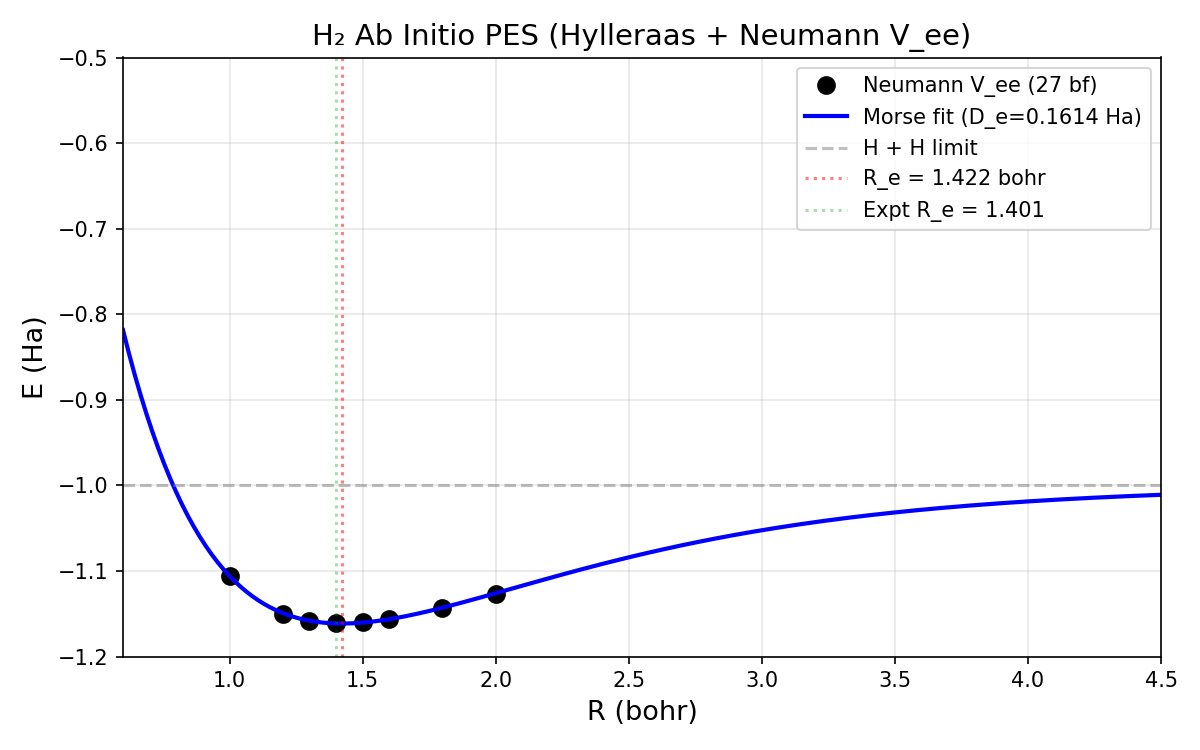
\includegraphics[width=\columnwidth]{../../benchmarks/ab_initio_nuclear/h2_pes_morse.png}
  \caption{Ab initio potential energy surface for H$_2$ computed
  from the Hylleraas basis with Neumann $V_{ee}$ (points) with Morse
  fit (solid curve).  The dissociation limit $E(\text{H} + \text{H}) =
  -1.0$~Ha is shown as a dashed line.  $D_e = 0.161$~Ha
  ($-7.5\%$ vs.\ experiment), $R_e = 1.42$~bohr ($+1.5\%$).}
  \label{fig:pes}
\end{figure}

%% ========================================================================
%% X. DISCUSSION
%% ========================================================================

\section{Discussion}
\label{sec:discussion}

\subsection{The universal structure of natural lattices}

Each natural geometry in the GeoVac hierarchy has the structure of a
fiber bundle over a radial base with angular fibers drawn from
representations of the rotation group---the universal pattern
identified in Paper~0~\cite{loutey_paper0}.  On $S^3$, the fibers
are SO(4) representations and the base is trivial; on the prolate
spheroid, the fibers are separated angular modes and the base is the
radial grid in $\xi$; on the hypersphere, the fibers are adiabatic
channel functions and the base is the hyperradial grid in $R$.

The transition from trivial bundles ($S^3$, prolate) to a non-trivial
bundle (hyperspherical) marks the point where the angular physics
\emph{depends on the radial coordinate}.  This is the signature of
the electron-electron cusp: its effective strength varies with $R$,
coupling the angular and radial degrees of freedom.

\subsection{Connection to quantum computing}

The lattice Hamiltonian's algebraic sparsity---enforced by angular
momentum selection rules via the Gaunt integrals~\eqref{eq:gaunt}---
has implications for quantum simulation.  In a companion study, we
compared the number of Pauli string terms after Jordan--Wigner
transformation for GeoVac lattice Hamiltonians versus conventional
Gaussian-basis Hamiltonians.  The GeoVac encoding scales as
$O(Q^{3.15})$ in the number of qubits $Q$, compared to
$O(Q^{4.60})$ for Gaussian bases, reflecting the structural sparsity
of the two-electron integral tensor (ERI density $\sim 1/M^2$
for the lattice versus $\sim O(1)$ for Gaussians).

\subsection{Open questions}

Several extensions are natural:
\begin{enumerate}
  \item \textbf{Coupled channels:} Adding the second adiabatic
    channel and computing the non-adiabatic coupling $P_{12}(R)$
    should reduce the error to $\sim$0.1\%~\cite{Macek1968}.
  \item \textbf{Three-electron systems:} Li requires a 9D
    configuration space with three hyperangles.  The adiabatic
    framework extends but the angular problem becomes significantly
    more complex.
  \item \textbf{Level 4 geometry:} The two-center, two-electron
    problem (H$_2$) likely requires a fibered product of prolate
    spheroidal and hyperspherical coordinates, with the bond length
    $R_{\mathrm{nuc}}$ as an additional slow variable.
  \item \textbf{Gauge structure:} The Berry connection
    $P_{\nu\mu}(R)$ on the fiber bundle of adiabatic channels is a
    prototype for understanding gauge fields on discrete
    lattices---connecting to the broader Geometric Vacuum program's
    investigation of emergent gauge structure.
\end{enumerate}

%% ========================================================================
%% XI. CONCLUSION
%% ========================================================================

\section{Conclusion}
\label{sec:conclusion}

The hyperspherical adiabatic solver achieves 0.05\% error for the
helium ground-state energy using a single adiabatic channel, a
$600 \times 600$ sparse matrix, and $\sim$3~seconds of runtime.
This is the most accurate GeoVac result for any two-electron system,
improving by a factor of 36 over the $S^3$ lattice (1.82\% error)
and by a factor of 34 over Full CI (1.71\% error) while using
matrices that are five orders of magnitude smaller.

The hyperspherical lattice extends the natural geometry principle to
multi-particle systems: it is structurally the same kind of object
as the atomic $S^3$ lattice and the molecular prolate spheroidal
lattice---a sparse graph with quantum number labels on nodes and
transition amplitudes on edges---but with the key generalization
that the angular structure (fiber) varies with the radial coordinate
(base), making it a non-trivial fiber bundle.

Combined with the prolate spheroidal electron lattice and the nuclear
lattice, the GeoVac framework produces ab initio rovibrational
frequencies for H$_2$ from first principles: $\omega_e =
4500$~cm$^{-1}$ ($+2.2\%$), $B_e = 59.1$~cm$^{-1}$ ($-2.9\%$),
with no experimental spectroscopic input at any stage.  The path
forward is clear: improve the electronic PES with larger CI spaces,
add coupled channels for sub-0.1\% atomic accuracy, and construct
the Level~4 geometry for full two-center, two-electron molecules.

\begin{acknowledgments}
This work was conducted independently with computational tools from
the GeoVac open-source project.
\end{acknowledgments}

%% ========================================================================
%% REFERENCES
%% ========================================================================

\begin{thebibliography}{99}

\bibitem{loutey_paper0}
J.~Loutey,
``Geometric Packing and the Universal Constant,''
GeoVac Paper~0 (2026).

\bibitem{loutey_paper1}
J.~Loutey,
``Spectral Graph Theory Foundations for Atomic Physics,''
GeoVac Paper~1 (2026).

\bibitem{loutey_paper7}
J.~Loutey,
``The Dimensionless Vacuum: Recovering the Schr\"odinger Equation
from Scale-Invariant Graph Topology,''
GeoVac Paper~7 (2026).

\bibitem{loutey_paper10}
J.~Loutey,
``The Nuclear Lattice: Rovibrational Spectra from SU(2) Algebraic
Chains,''
GeoVac Paper~10 (2026).

\bibitem{loutey_paper11}
J.~Loutey,
``The Molecular Fock Projection: Diatomic Molecules as Prolate
Spheroidal Lattices,''
GeoVac Paper~11 (2026).

\bibitem{loutey_paper12}
J.~Loutey,
``Algebraic Two-Electron Integrals on the Prolate Spheroidal
Lattice,''
GeoVac Paper~12 (2026).

\bibitem{Fock1935}
V.~Fock,
``Zur Theorie des Wasserstoffatoms,''
Z. Phys. \textbf{98}, 145--154 (1935).

\bibitem{Fock1954}
V.~Fock,
``On the Schr\"odinger equation of the helium atom,''
Izv. Akad. Nauk SSSR Ser. Fiz. \textbf{18}, 161--172 (1954).

\bibitem{Macek1968}
J.~Macek,
``Properties of autoionizing states of He,''
J. Phys. B \textbf{1}, 831--843 (1968).

\bibitem{Lin1995}
C.~D. Lin,
``Hyperspherical coordinate approach to atomic and other Coulombic
three-body systems,''
Phys. Rep. \textbf{257}, 1--83 (1995).

\bibitem{KlarKlar1980}
H.~Klar and M.~Klar,
``An accurate treatment of two-electron systems,''
J. Phys. B \textbf{13}, 1057--1072 (1980).

\bibitem{Pekeris1958}
C.~L. Pekeris,
``Ground state of two-electron atoms,''
Phys. Rev. \textbf{112}, 1649--1658 (1958).

\bibitem{Kato1957}
T.~Kato,
``On the eigenfunctions of many-particle systems in quantum
mechanics,''
Commun. Pure Appl. Math. \textbf{10}, 151--177 (1957).

\bibitem{Berry1984}
M.~V. Berry,
``Quantal phase factors accompanying adiabatic changes,''
Proc. R. Soc. London A \textbf{392}, 45--57 (1984).

\bibitem{Mead1992}
C.~A. Mead,
``The geometric phase in molecular systems,''
Rev. Mod. Phys. \textbf{64}, 51--85 (1992).

\bibitem{Varshalovich1988}
D.~A. Varshalovich, A.~N. Moskalev, and V.~K. Khersonskii,
\textit{Quantum Theory of Angular Momentum}
(World Scientific, Singapore, 1988).

\bibitem{Herzberg1950}
G.~Herzberg,
\textit{Spectra of Diatomic Molecules}
(Van Nostrand, New York, 1950).

\bibitem{NIST_H2}
National Institute of Standards and Technology,
``Diatomic Spectral Database --- H$_2$,''
\url{https://www.nist.gov/pml/diatomic-spectral-database}.

\end{thebibliography}

\end{document}
